\section{Результаты}

\subsection{Описательная статистика}

Выборка HotpotQA --- 600 вопросов: по 200 уровней easy, medium, hard; 504 вопроса типа bridge и 96 типа comparison. Корпус HotpotQA --- 5\,904 абзаца, SQuAD --- 2\,067 абзацев. Число чанков приведено в таблице~\ref{tab:corpus}.

\begin{gosttable}{Корпуса и вопросы}\label{tab:corpus}
\begin{tabular}{lrrrrrr}
\toprule
Датасет & Абзацев & \multicolumn{3}{c}{Чанков при размере, слов} & Длина вопроса, & Пересечение \\
 & & 50 & 100 & 200 & слов (медиана) & с эталоном\footnotemark \\
\midrule
HotpotQA & 5\,904 & 14\,659 & 8\,136 & 6\,097 & 17 & 0,823 \\
SQuAD & 2\,067 & 6\,859 & 3\,630 & 2\,222 & 10 & 0,670 \\
\bottomrule
\end{tabular}
\end{gosttable}
\footnotetext{Доля значимых слов вопроса (без стоп-слов), встречающихся в эталонных абзацах; среднее по вопросам.}

Таблица~\ref{tab:desc} --- метрики базовой конфигурации: чанк 100 слов, top-5. В квадратных скобках --- 95\,\% бутстреп-интервал (2\,000 повторов).

\begin{gosttable}{Качество поиска и ответа в базовой конфигурации (чанк 100, top-5)}\label{tab:desc}
\begin{tabular}{llccc}
\toprule
Датасет & Ретривер & Полнота поиска & F1 ответа & Доля правильных \\
\midrule
\inputtab tables/tab_desc.tex 
\bottomrule
\end{tabular}
\end{gosttable}

Стандартное отклонение F1 --- от 0,46 на HotpotQA до 0,36--0,38 на SQuAD, медиана F1 на SQuAD равна 1 у всех ретриверов. Распределение F1 бимодально (рисунок~\ref{fig:dist}): у HotpotQA (гибрид) 42,3\,\% ответов имеют F1~=~0 и 41,2\,\% --- F1~=~1, у SQuAD --- 14,0\,\% и 75,7\,\%. Тест Шапиро--Уилка по всем 600 вопросам отвергает нормальность с $p < 10^{-29}$ в обоих наборах. Поэтому для F1 дальше используются ранговые тесты, а для бинарной правильности --- тесты для долей.

\begin{figure}[ht]
\centering
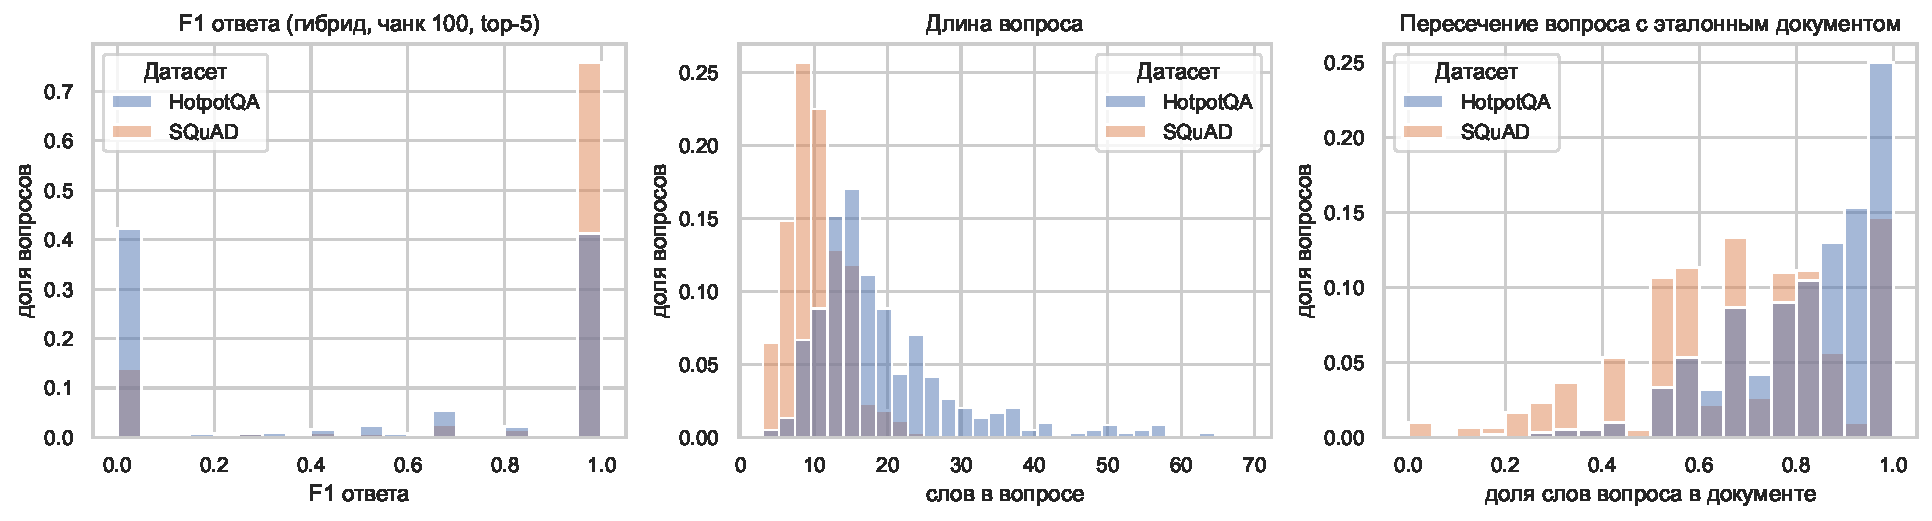
\includegraphics[width=\linewidth]{figures/distributions.pdf}
\caption{Распределения F1 ответа, длины вопроса и лексического пересечения}\label{fig:dist}
\end{figure}

HotpotQA сложнее SQuAD по всем метрикам: при гибридном поиске F1 0,503 против 0,817. При этом ответ присутствует в найденном контексте у 79,7\,\% вопросов HotpotQA и 96,2\,\% вопросов SQuAD. Полные таблицы по 72 конфигурациям --- в приложении~\ref{app:grid}.

\subsection{Проверка гипотез}

Сводка --- в таблице~\ref{tab:hyp}. Для парных сравнений (один вопрос во всех конфигурациях) база --- чанк 100 и top-5, для H2 и H3 ретривер фиксирован --- гибрид. Уровень значимости 0,05, попарные сравнения с поправкой Холма. Для F1 и полноты HotpotQA (значения 0; 0,5; 1) --- знаково-ранговый тест Вилкоксона с отбрасыванием нулевых разностей, для бинарных метрик (полнота SQuAD, попадание, правильность) --- тест Мак-Немара. Для каждой пары приведена средняя парная разность и ее бутстреп-интервал.

\begin{gosttable}{Результаты проверки гипотез}\label{tab:hyp}
\begin{tabular}{>{\raggedright\arraybackslash}p{0.7cm}>{\raggedright\arraybackslash}p{2.8cm}>{\raggedright\arraybackslash}p{4.5cm}>{\raggedright\arraybackslash}p{3.5cm}>{\raggedright\arraybackslash}p{2.8cm}}
\toprule
№ & Тест & HotpotQA & SQuAD & Вывод \\
\midrule
H1 & Фридман, Q Кохрена & полнота: $\chi^2 = 170{,}9$, $p < 10^{-37}$, $W = 0{,}14$; F1: $\chi^2 = 31{,}7$, $p = 1{,}3 \cdot 10^{-7}$, $W = 0{,}03$ & полнота: $p = 4{,}5 \cdot 10^{-5}$; F1: $p = 0{,}049$, гибрид лучше BM25 на 0,026 & подтверждена; на SQuAD эффект на ответ мал \\
H2 & тренд Пейджа, парная разность $k{=}10$ и $k{=}5$ & полнота: $+0{,}084$, $p < 10^{-21}$; F1: $-0{,}003$ [$-0{,}024$; $0{,}018$] & полнота: $+0{,}028$, $p = 10^{-4}$; F1: $-0{,}010$ [$-0{,}024$; $0{,}004$] & рост F1 после $k{=}5$ не выше 0,018 \\
H3 & Фридман, Q Кохрена & F1: $p = 0{,}66$; полнота: $p = 3{,}4 \cdot 10^{-11}$ & F1: $p = 0{,}23$; полнота: $p = 8{,}6 \cdot 10^{-5}$ & для F1 не подтверждена \\
H4 & Манн--Уитни, Краскел--Уоллис, $\chi^2$ & comparison хуже bridge, $p = 0{,}004$; easy лучше medium и hard, $p_{Holm} = 1{,}3 \cdot 10^{-6}$ & --- & частично \\
H5 & точный тест Фишера & отношение шансов 55, $p < 10^{-39}$ & отношение шансов 40, $p < 10^{-13}$ & подтверждена \\
H6 & Вилкоксон, Мак-Немар, Фридман, GEE & полнота на шаге 2: 0,916 против 0,871, $p_{Holm} = 1{,}7 \cdot 10^{-8}$; F1 не меняется & полнота на шаге 4 ниже: 0,970 против 0,987, $p_{Holm} = 0{,}028$; F1 как у одношагового & подтверждена для поиска; на SQuAD итерации снижают полноту \\
\bottomrule
\end{tabular}
\end{gosttable}

\textbf{H1, ретривер.} На HotpotQA плотный поиск превосходит BM25 по полноте на 12,8 пункта (0,866 против 0,738, интервал разности [0,107; 0,152], Вилкоксон $p_{Holm} = 2{,}7 \cdot 10^{-24}$) и по F1 на 5,8 пункта ([0,035; 0,082], $p_{Holm} = 8{,}5 \cdot 10^{-6}$). Плотный поиск находит больше гибрида (разность полноты 0,026, $p = 0{,}001$), но по F1 они не различаются ($p = 0{,}21$). На SQuAD тип ретривера меняет полноту: гибрид 0,953 против 0,905 у BM25 (Мак-Немар $p_{Holm} = 5{,}9 \cdot 10^{-5}$). По F1 значима одна пара: гибрид лучше BM25 на 0,026 ([0,007; 0,045], Вилкоксон $p_{Holm} = 0{,}031$); по бинарной правильности та же пара на грани (Мак-Немар $p_{Holm} = 0{,}064$, Q Кохрена $p = 0{,}052$). Омнибусный тест Фридмана для F1 SQuAD ($p = 0{,}049$) не выдерживает поправки Холма на четыре омнибусных теста H1, поэтому решение по SQuAD опирается на парную разность с интервалом: эффект на ответ есть, но мал и вдвое меньше, чем на HotpotQA. Размер эффекта по Кендаллу\footnote{Коэффициент согласованности $W = \chi^2_F / (n(k-1))$, где $\chi^2_F$ --- статистика Фридмана, $n$ --- число вопросов, $k$ --- число уровней фактора; от 0 до 1. Для HotpotQA и полноты: $170{,}9 / (600 \cdot 2) = 0{,}14$.} малый: от 0,005 до 0,14.

\textbf{H2, top-k.} Полнота растет на всем диапазоне: у HotpotQA 0,423, 0,744, 0,840, 0,924 при $k$ = 1, 3, 5, 10, у SQuAD 0,790, 0,928, 0,953, 0,982; прирост от $k = 5$ к $k = 10$ значим в обоих наборах (Вилкоксон $p < 10^{-21}$, Мак-Немар $p = 10^{-4}$). F1 растет только до $k = 3$--5: 0,378, 0,485, 0,503, 0,499. Незначимость разницы F1 между $k = 5$ и $k = 10$ сама по себе плато не доказывает, поэтому дан интервал парной разности: $-0{,}003$ [$-0{,}024$; $0{,}018$] на HotpotQA и $-0{,}010$ [$-0{,}024$; $0{,}004$] на SQuAD. Прирост F1 больше 0,018 и 0,004 соответственно отвергается односторонне на уровне 97,5\,\% (верхняя граница двустороннего 95\,\% интервала). Эквивалентность в пределах $\pm 0{,}02$ (TOST, 90\,\% интервал) формально не подтверждена: нижние границы $-0{,}021$ и $-0{,}022$ выходят за предел на тысячные. Рост полноты после $k = 5$ не переходит в качество ответа (рисунок~\ref{fig:topk}).

\begin{figure}[ht]
\centering
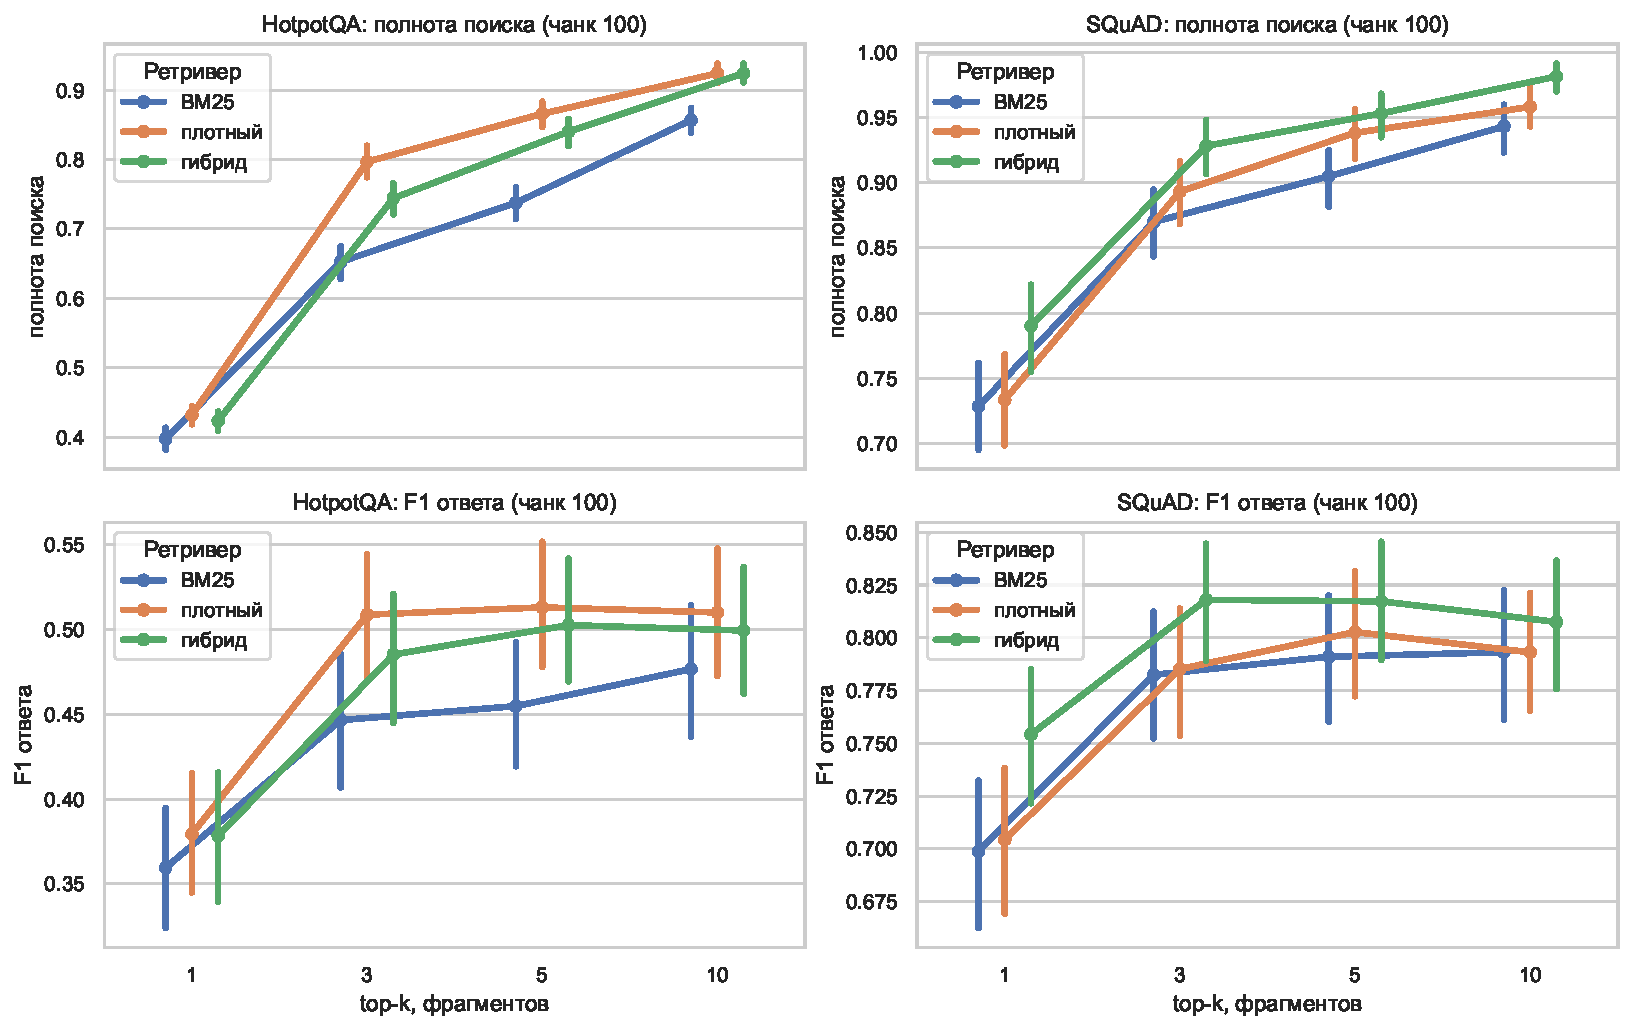
\includegraphics[width=0.92\linewidth]{figures/topk_curves.pdf}
\caption{Полнота поиска и F1 ответа в зависимости от top-k, чанк 100 слов, 95\,\% интервал}\label{fig:topk}
\end{figure}

\textbf{H3, размер чанка.} Крупные чанки повышают полноту: у HotpotQA 0,802, 0,840, 0,852 при 50, 100, 200 словах, у SQuAD 0,932, 0,953, 0,967. На F1 в парном тесте эффект не значим (HotpotQA 0,484, 0,503, 0,498). В регрессии по всей сетке эффект чанка значим, но мал: $\pm 0{,}01$ F1 (раздел~\ref{sec:reg}).

\textbf{H4, свойства вопроса.} Направление по типу вопроса обратно ожидаемому: comparison хуже bridge (F1 0,384 против 0,525, $n$ = 96 и 504, Манн--Уитни $p = 0{,}004$, рангово-бисериальная корреляция $-0{,}17$, знак минус означает перевес bridge). Тип вопроса распределен по уровням почти равномерно (comparison: 32, 29, 35 вопросов на easy, medium, hard), и с поправкой на уровень эффект сохраняется: $-0{,}142$ F1, $p = 0{,}005$ (МНК с ошибками HC3). Вопросы с ответом yes/no исключены из выборки; в train-части HotpotQA это 31\,\% comparison-вопросов (5\,481 из 17\,456), у bridge таких нет. Оставшиеся comparison-вопросы --- выбор одного из двух объектов, и вывод относится только к ним. Уровень сложности значим (Краскел--Уоллис $H = 33{,}6$, $p = 5{,}1 \cdot 10^{-8}$, $\varepsilon^2 = 0{,}056$; $\chi^2 = 26{,}7$ для доли правильных, V Крамера 0,21). Отличается только easy (F1 0,653) от medium (0,422) и hard (0,432), $p_{Holm} = 1{,}3 \cdot 10^{-6}$; medium и hard не различаются ($p = 0{,}92$).

\textbf{H5, ответ в контексте.} Если ответа в найденных чанках нет, правильных ответов почти нет: 3,3\,\% у HotpotQA и 13,0\,\% у SQuAD (последние --- частичные совпадения при F1~$\ge 0{,}5$). Если ответ в контексте есть, правильно отвечено 65,3\,\% и 85,8\,\% вопросов. Значит, у HotpotQA около трети ошибок при найденном ответе приходится на ридер, а не на поиск. На SQuAD релевантным считается чанк, содержащий ответ (раздел 4.3), поэтому там <<ответ в контексте>> почти совпадает с попаданием поиска, и для SQuAD H5 проверяет в основном ридер.

\textbf{H6, итерации} --- в разделе~\ref{sec:iter}.

\subsection{Корреляции параметров и метрик}

Корреляции Спирмена по всей сетке (21\,600 строк на датасет) показаны на рисунке~\ref{fig:corr}, ключевые пары --- в таблице~\ref{tab:corr}.

\begin{gosttable}{Корреляции Спирмена ключевых пар}\label{tab:corr}
\begin{tabular}{llrr}
\toprule
Параметр или свойство & Метрика & HotpotQA & SQuAD \\
\midrule
top-k & полнота поиска & 0,575 & 0,220 \\
top-k & F1 ответа & 0,087 & 0,061 \\
размер чанка & F1 ответа & 0,022 & 0,021 \\
слов в контексте & F1 ответа & 0,090 & 0,076 \\
длина вопроса & F1 ответа & 0,196 & 0,032 \\
лексическое пересечение & полнота поиска & 0,098 & 0,230 \\
лексическое пересечение & F1 ответа & 0,242 & 0,223 \\
оценка ретривера за первый чанк\footnotemark & полнота поиска & 0,099 & 0,265 \\
полнота поиска & F1 ответа & 0,328 & 0,566 \\
уверенность ридера & правильность & 0,369 & 0,475 \\
\bottomrule
\end{tabular}
\end{gosttable}
\footnotetext{Перцентиль оценки внутри ретривера и размера чанка: шкалы BM25, косинуса и RRF несравнимы.}

Все пары значимы после поправки Холма, но строки одного вопроса зависимы, поэтому $p$-значения здесь занижены и служат только описанием. Значимость проверена регрессией с кластерными ошибками. Параметры системы коррелируют с F1 слабо ($|\rho| < 0{,}1$), а свойства вопроса (пересечение, длина) и полнота поиска --- сильнее. Связь полноты и F1 на HotpotQA ($\rho = 0{,}33$) слабее, чем на SQuAD ($0{,}57$), но напрямую эти числа не сравнимы: на SQuAD релевантный чанк по определению содержит ответ, на HotpotQA --- опорное предложение. Внутри HotpotQA найденные нужные документы объясняют лишь часть качества ответа.

\begin{figure}[ht]
\centering
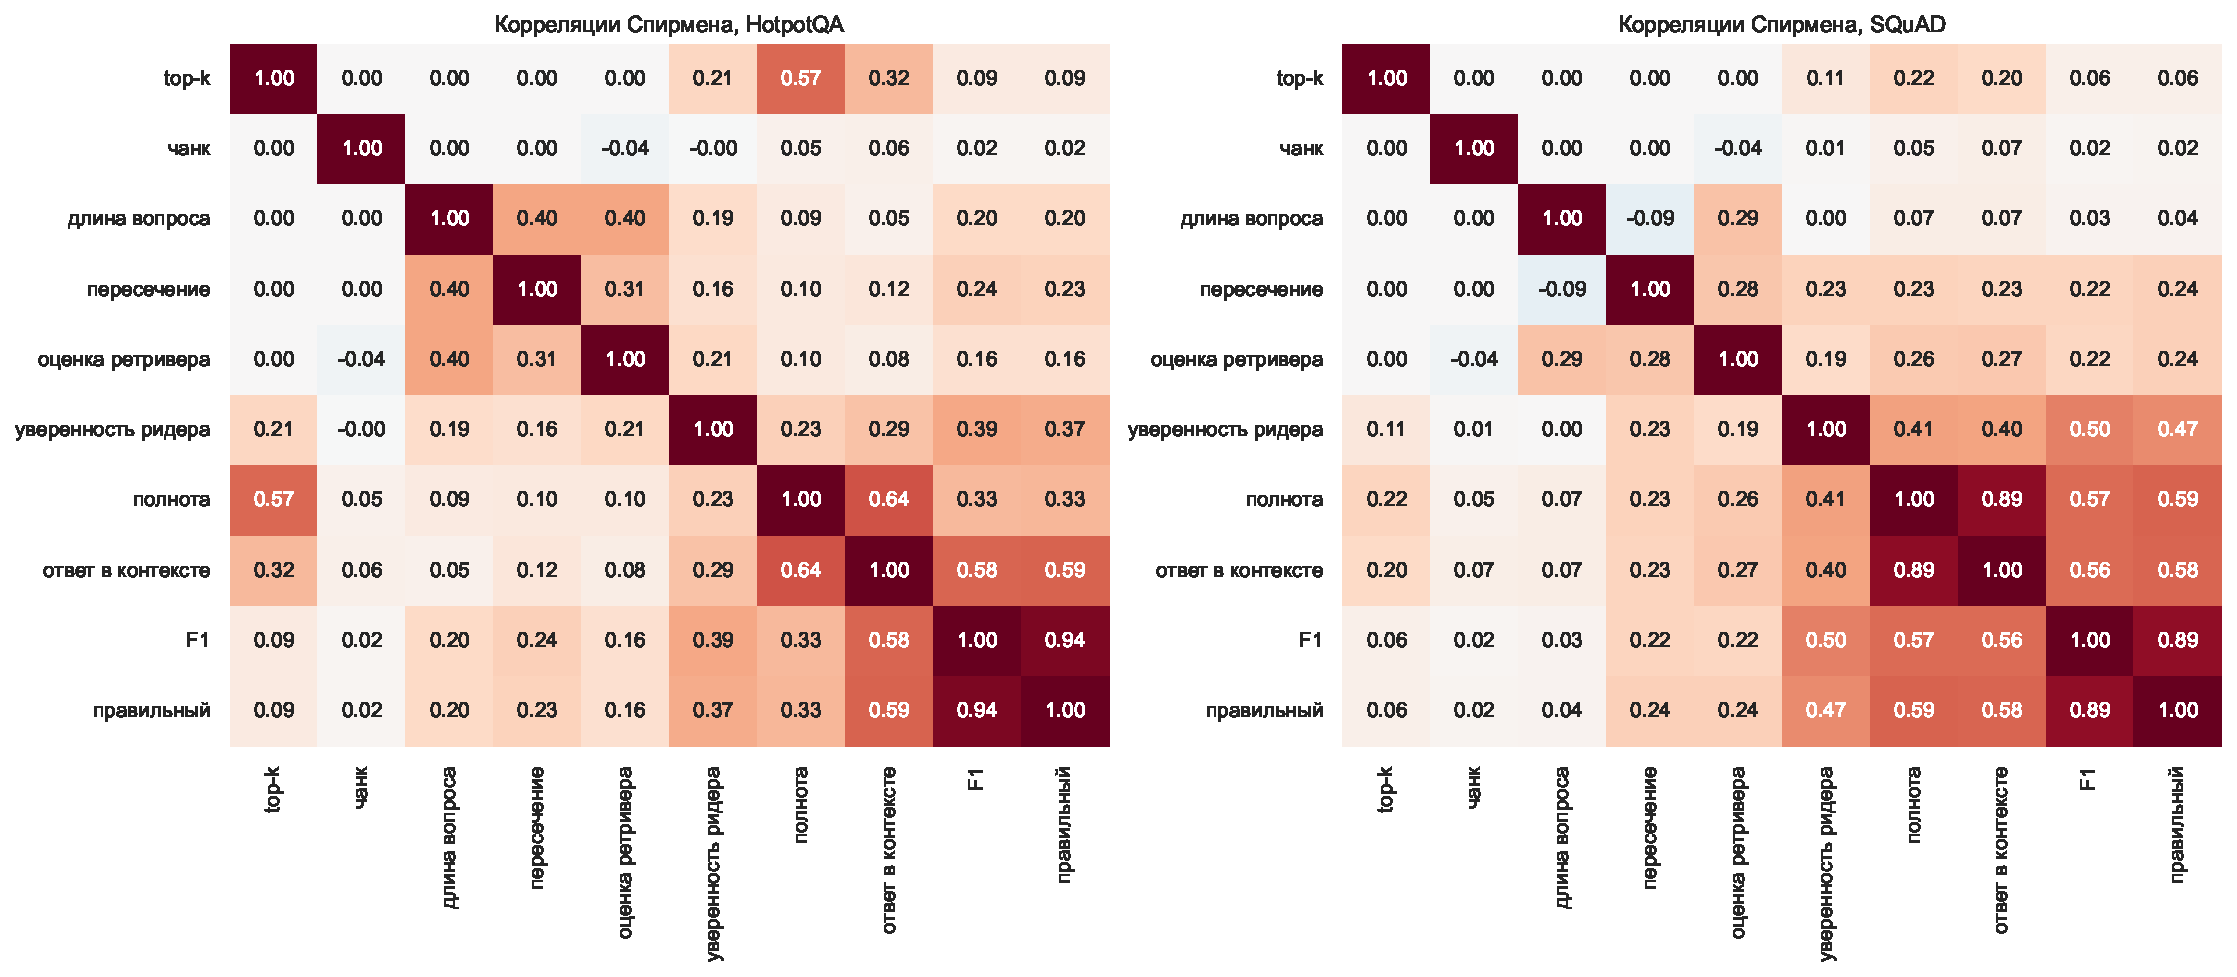
\includegraphics[width=\linewidth]{figures/spearman.pdf}
\caption{Матрицы корреляций Спирмена параметров и метрик}\label{fig:corr}
\end{figure}

\subsection{Регрессия качества по параметрам}\label{sec:reg}

Модель: F1 по ретриверу, датасету, $\log_2$ top-k, размеру чанка, длине вопроса, лексическому пересечению и числовому ответу; взаимодействия ретривера и top-k с датасетом. МНК, ошибки кластеризованы по вопросу (1\,200 кластеров, 43\,200 наблюдений). Коэффициенты --- в таблице~\ref{tab:ols}, база --- BM25, HotpotQA, чанк 100.

\begin{gosttable}{Регрессия F1 ответа, МНК с кластерными ошибками}\label{tab:ols}
\begin{tabular}{lrrr}
\toprule
Фактор & Коэффициент & 95\,\% интервал & $p$ \\
\midrule
Плотный ретривер & 0,043 & [0,027; 0,058] & $< 0{,}001$ \\
Гибридный ретривер & 0,030 & [0,021; 0,039] & $< 0{,}001$ \\
Плотный $\times$ SQuAD & $-0{,}034$ & [$-0{,}057$; $-0{,}011$] & 0,004 \\
Удвоение top-k ($\log_2 k$) & 0,037 & [0,029; 0,046] & $< 0{,}001$ \\
$\log_2 k$ $\times$ SQuAD & $-0{,}016$ & [$-0{,}026$; $-0{,}005$] & 0,004 \\
Чанк 50 слов & $-0{,}011$ & [$-0{,}022$; $-0{,}0004$] & 0,042 \\
Чанк 200 слов & 0,012 & [0,004; 0,019] & 0,002 \\
SQuAD & 0,507 & [0,462; 0,553] & $< 0{,}001$ \\
Длина вопроса, слово & 0,007 & [0,005; 0,009] & $< 0{,}001$ \\
Лексическое пересечение, 0 $\to$ 1 & 0,490 & [0,395; 0,586] & $< 0{,}001$ \\
Числовой ответ & $-0{,}062$ & [$-0{,}106$; $-0{,}019$] & 0,005 \\
\bottomrule
\end{tabular}
\end{gosttable}

$R^2 = 0{,}206$. Главное в разложении дисперсии: внутри одного датасета параметры системы (ретривер, top-k, чанк) объясняют 1,1\,\% дисперсии F1 на HotpotQA и 0,7\,\% на SQuAD, а фиксированный эффект вопроса --- 68\,\% и 60\,\%. Качество определяет прежде всего вопрос, параметры двигают среднее на единицы пунктов. Самый сильный фактор --- лексическое пересечение: рост на 0,1 добавляет 0,049 F1.

Логистическая модель правильности (GEE, обменная корреляция внутри вопроса) дает те же знаки: отношение шансов гибрида к BM25 1,20 [1,15; 1,25], плотного 1,15 [1,08; 1,23], на удвоение top-k 1,18 [1,14; 1,22], на чанк 200 против 100 --- 1,06 [1,02; 1,11]. Мультиколлинеарность низкая: VIF по матрице плана модели без взаимодействий не выше 1,43. Остатки МНК ненормальны из-за бимодальности F1 (приложение~\ref{app:diag}), поэтому выводы о значимости опираются на кластерные ошибки и GEE, а не на нормальную теорию.

\subsection{Классификация <<правильный/неправильный>>}

Задача --- предсказать правильность ответа (F1~$\ge 0{,}5$) по логу. Признаки берутся только из того, что система знает без эталона: параметры конфигурации, датасет, длина вопроса, число слов в контексте, перцентили оценок ретривера. Лексическое пересечение и числовой ответ сюда не входят: оба считаются по эталону. Три набора: <<до ридера без датасета>>, <<до ридера>> и <<с ридером>> (плюс уверенность ридера и ранг чанка с ответом). Проверка --- 5-кратная групповая кросс-валидация: все конфигурации одного вопроса в одном фолде.

\begin{gosttable}{Качество классификации правильности ответа, out-of-fold}\label{tab:clf}
\begin{tabular}{llrrrr}
\toprule
Модель & Признаки & ROC-AUC & PR-AUC & Accuracy & Брайер \\
\midrule
Всегда <<правильный>> & --- & 0,500 & 0,635 & 0,635 & 0,232 \\
Логит-регрессия & до ридера без датасета & 0,637 & 0,740 & 0,654 & 0,220 \\
Бустинг & до ридера без датасета & 0,711 & 0,794 & 0,681 & 0,205 \\
Логит-регрессия & до ридера & 0,737 & 0,808 & 0,695 & 0,195 \\
Бустинг & до ридера & 0,747 & 0,820 & 0,699 & 0,194 \\
Логит-регрессия & с ридером & 0,835 & 0,896 & 0,762 & 0,159 \\
Бустинг & с ридером & 0,837 & 0,886 & 0,766 & 0,159 \\
\bottomrule
\end{tabular}
\end{gosttable}

Результаты (таблица~\ref{tab:clf}, рисунок~\ref{fig:clf}): до ответа ридера правильность предсказуема с ROC-AUC 0,74--0,75, и большая часть этого --- знание датасета: без него 0,64 у логистической регрессии и 0,71 у бустинга. Уверенность ридера поднимает ROC-AUC до 0,84. По перестановочной важности главный признак --- уверенность ридера (падение ROC-AUC на 0,211), затем датасет (0,039), ранг чанка с ответом (0,028), длина вопроса (0,021) и перцентиль оценки ретривера (0,011); параметры конфигурации дают меньше 0,002 каждый. В логистической регрессии до ридера наибольший по модулю стандартизованный коэффициент --- у датасета ($-0{,}90$ для HotpotQA), затем перцентиль оценки ретривера (0,39) и длина вопроса (0,26).

\begin{figure}[ht]
\centering
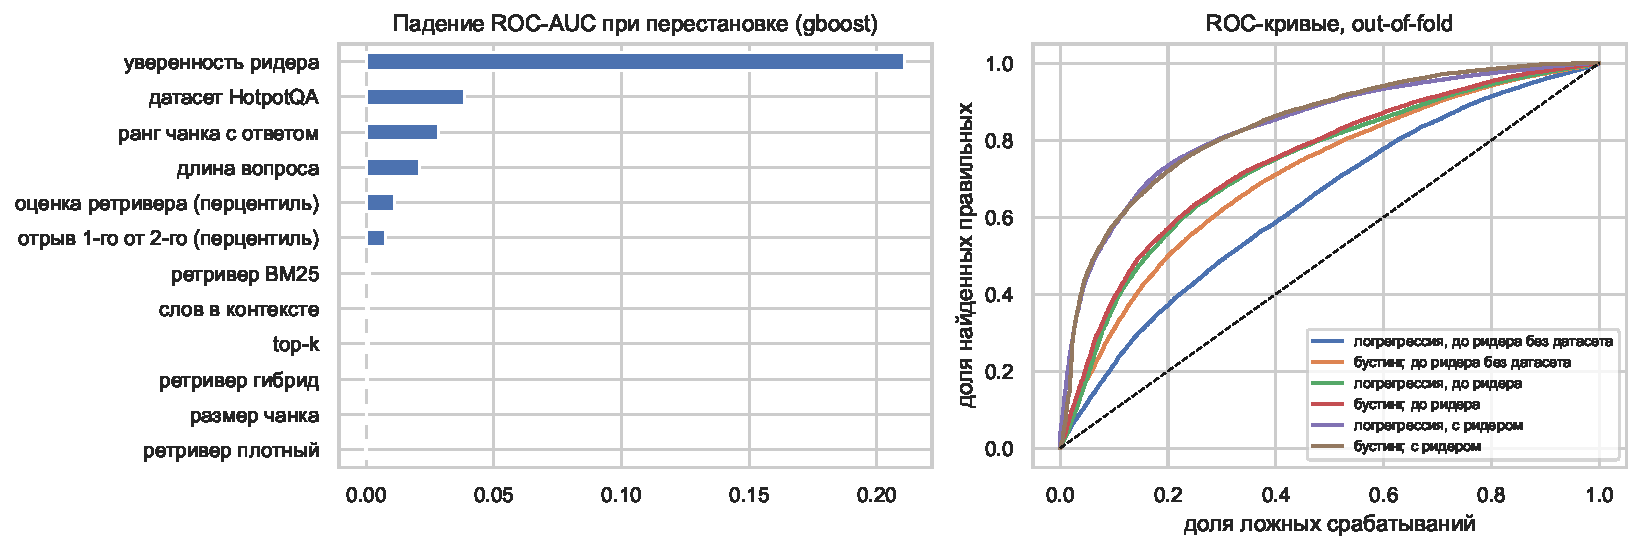
\includegraphics[width=0.95\linewidth]{figures/classification.pdf}
\caption{Перестановочная важность признаков и ROC-кривые}\label{fig:clf}
\end{figure}

\subsection{Динамика по итерациям поиска}\label{sec:iter}

\begin{gosttable}{Полнота и F1 по шагам итеративного поиска и при одношаговом поиске того же объема}\label{tab:iter}
\begin{tabular}{lrrrrrr}
\toprule
Датасет & Шаг & Чанков & \multicolumn{2}{c}{Полнота поиска} & \multicolumn{2}{c}{F1 ответа} \\
 & & & итеративный & одношаговый & итеративный & одношаговый \\
\midrule
\inputtab tables/tab_iterations.tex 
\bottomrule
\end{tabular}
\end{gosttable}

Средние по шагам --- в таблице~\ref{tab:iter}. Сравнение режимов на каждом шаге: Вилкоксон для F1 и полноты HotpotQA, Мак-Немар для бинарной полноты SQuAD, поправка Холма на три шага. На HotpotQA итеративный поиск находит нужные документы быстрее: на шаге 2 полнота 0,916 против 0,871 при одношаговом поиске того же объема (разность 0,045 [0,031; 0,059], $p_{Holm} = 1{,}7 \cdot 10^{-8}$), на шаге 3 --- 0,948 против 0,913 ($p_{Holm} = 2{,}2 \cdot 10^{-8}$), на шаге 4 --- 0,954 против 0,940 ($p_{Holm} = 0{,}011$). F1 по шагам на HotpotQA не меняется (Фридман $p = 0{,}17$, изменение с шага 1 на шаг 4 $+0{,}017$ [$-0{,}010$; $0{,}043$]).

На SQuAD итерации снижают полноту: на шаге 4 она 0,970 против 0,987 у одношагового поиска (Мак-Немар $p_{Holm} = 0{,}028$), на шаге 3 --- 0,963 против 0,978 ($p = 0{,}039$, после поправки $0{,}078$). F1 на SQuAD падает с ростом контекста в обоих режимах: в итеративном на 0,024 [0,007; 0,041] с шага 1 до шага 4 (Фридман $p = 0{,}0009$), в одношаговом на 0,015 [$-0{,}003$; 0,034]. На одном шаге режимы по F1 не различаются ($p_{Holm} \ge 0{,}70$), то есть итерации сами по себе F1 не снижают. Тест Пейджа односторонний и проверяет рост, поэтому падение видно по Фридману и бутстреп-интервалу.

GEE для правильности посчитан отдельно по датасетам, так как динамика в них разная. HotpotQA: отношение шансов на шаг 1,01 ($p = 0{,}51$), взаимодействие шага с режимом $p = 0{,}20$. SQuAD: 0,96 на шаг ($p = 0{,}067$), взаимодействие $p = 0{,}25$. Значимого влияния шага и различия режимов по правильности нет ни в одном наборе (рисунок~\ref{fig:iter}).

\begin{figure}[ht]
\centering
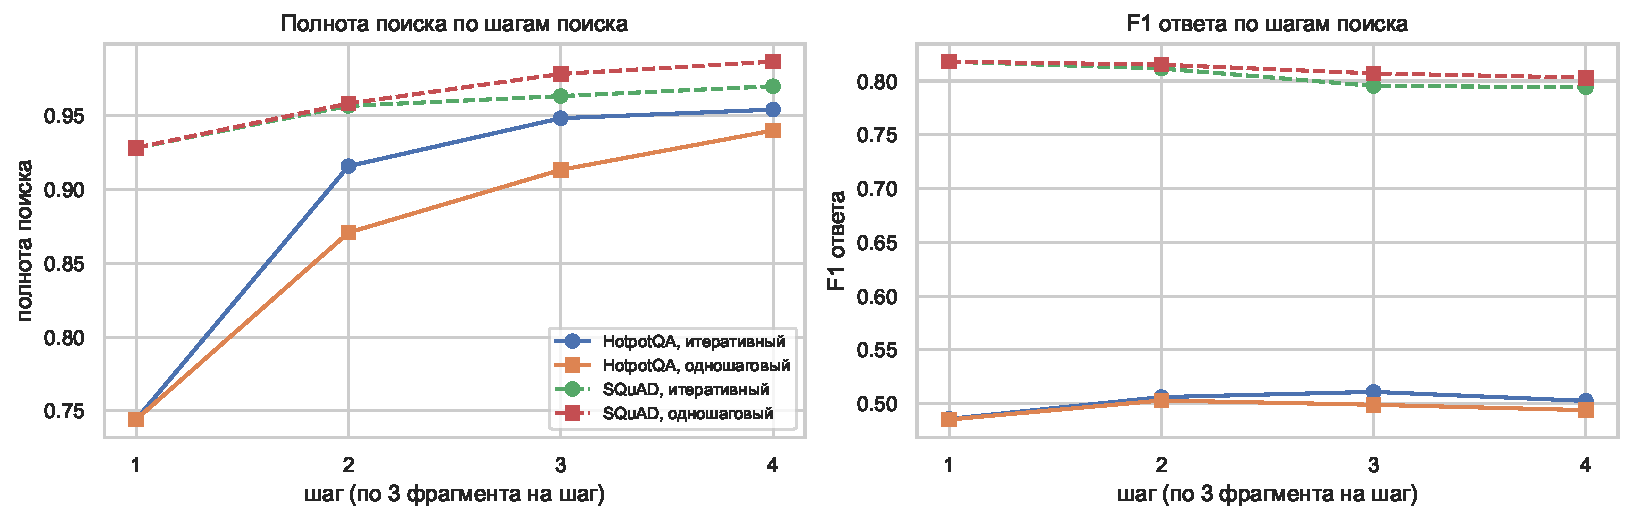
\includegraphics[width=\linewidth]{figures/iterations.pdf}
\caption{Полнота поиска и F1 ответа по шагам}\label{fig:iter}
\end{figure}

\section{Обсуждение и ограничения}

Параметры RAG значимо влияют на поиск: тип ретривера, top-k, размер чанка и итерации меняют полноту на 4--50 пунктов. На ответ они влияют на единицы пунктов, а прирост F1 после $k = 5$ не превышает 0,018. На одношаговых вопросах итерации снижают полноту, а F1 падает с ростом контекста в обоих режимах. Разброс качества определяется вопросом: его лексической близостью к документу, сложностью и типом. Отсюда практический вывод: сравнивать конфигурации RAG нужно парными тестами на одних вопросах. Межгрупповое сравнение средних тонет в разбросе между вопросами, который в 60--90 раз больше эффекта параметров.

На HotpotQA плотный поиск сильнее BM25, тогда как в BEIR~\cite{beir} BM25 часто сильнее плотных моделей вне домена обучения. Предобучение e5 включает пары текстов из Википедии, а дообучение --- MS MARCO и Natural Questions~\cite{e5}; пересечение этих данных с текстами HotpotQA и SQuAD не исключено, поэтому вывод о преимуществе e5 относится к корпусам этой работы.

\textbf{Ограничения.}
\begin{itemize}
\item Ридер экстрактивный (roberta-base-squad2), а не генеративная LLM. Выводы о потолке качества относятся к этому ридеру. Он обучен на SQuAD 2.0 train, куда входят вопросы SQuAD 1.1 train, поэтому на SQuAD он работает в своем домене и F1 там завышен относительно HotpotQA.
\item Корпус HotpotQA --- 5\,904 абзаца выбранных вопросов, а не вся Википедия. Абсолютная полнота выше, чем в открытой постановке; сравнения внутри сетки от этого не зависят.
\item Порог правильности F1~$\ge 0{,}5$ условный. Он засчитывает частичные совпадения, отсюда 13\,\% <<правильных>> ответов на SQuAD без ответа в контексте.
\item Корреляции и $p$-значения раздела 5.3 посчитаны по зависимым строкам и служат описанием.
\item Релевантность определена по-разному: на HotpotQA --- чанк с опорным предложением, на SQuAD --- чанк исходного абзаца с ответом. Полнота поиска на двух наборах поэтому не сравнима напрямую.
\item Вопросы HotpotQA взяты из train-части: dev-часть содержит только уровень hard. Ридер на HotpotQA не обучался.
\item Лексическое пересечение считается по эталонному документу. Это свойство вопроса для анализа, а не признак, доступный работающей системе; в классификацию оно не входит.
\item Comparison-вопросов 96, интервал для этой группы широкий.
\item Итерации --- шаги одного многошагового поиска, а не версии системы во времени. Глубина слияния RRF в итеративном и одношаговом режимах разная (60 и 50), отсюда расхождение F1 на шаге 1 в третьем знаке.
\item Плотная модель одна (e5-small-v2), размер выборки --- 600 вопросов на датасет, зерно одно.
\end{itemize}

\section{Выводы}

\begin{enumerate}
\item На HotpotQA и SQuAD прогнана система RAG по сетке из 72 конфигураций: 43\,200 строк лога ответов и 108\,000 строк лога поиска.
\item Тип ретривера значимо влияет на полноту поиска в обоих наборах и на F1: на HotpotQA плотный поиск лучше BM25 на 5,8 пункта, на SQuAD гибрид лучше BM25 на 2,6 пункта.
\item Полнота растет с top-k до $k = 10$, а прирост F1 от $k = 5$ к $k = 10$ не превышает 0,018 на HotpotQA и 0,004 на SQuAD (верхняя граница 95\,\% интервала).
\item Размер чанка влияет на полноту поиска, на F1 --- в пределах 0,01.
\item Внутри датасета параметры системы объясняют около 1\,\% дисперсии F1, вопрос --- 60--68\,\%. Сильнейший фактор --- лексическое пересечение вопроса и документа.
\item Правильность ответа предсказуема по логу без эталона с ROC-AUC 0,74--0,75 до ридера и 0,84 с его уверенностью.
\item Итеративный поиск повышает полноту на многошаговых вопросах на 4,5 пункта на шаге 2, а на одношаговых снижает ее к шагу 4 на 1,7 пункта. На F1 итерации сами по себе не влияют ни в одном наборе.
\end{enumerate}
